\chapter{前言}
\renewcommand{\baselinestretch}{10.0} %設定行距
\pagenumbering{arabic} %設定頁號阿拉伯數字
\setcounter{page}{1}  %設定頁數
\fontsize{14pt}{2.5pt}\sectionef
\section{研究動機}
機器學習與各領域結合的應用越來越廣泛,在機電系統採用強化學習是為了讓機電系統的控制達到最佳化。本專題以實體的冰球機(圖.\ref{fig.冰球機})之機電系統作為訓練模型,將實體機器轉移到虛擬環境(圖.\ref{fig.模擬冰球機})進行模擬,為了找到適合的演算方式,因此將模型簡化(圖.\ref{fig.pong_gym})後再進行測試各種算法的優劣,透過不斷的訓練來得到一個優化過的對打系統。\\

\begin{figure}[hbt!]
\begin{center}
\subfigure{
\begin{minipage}[t]{0.3\linewidth}  %設定圖片間距
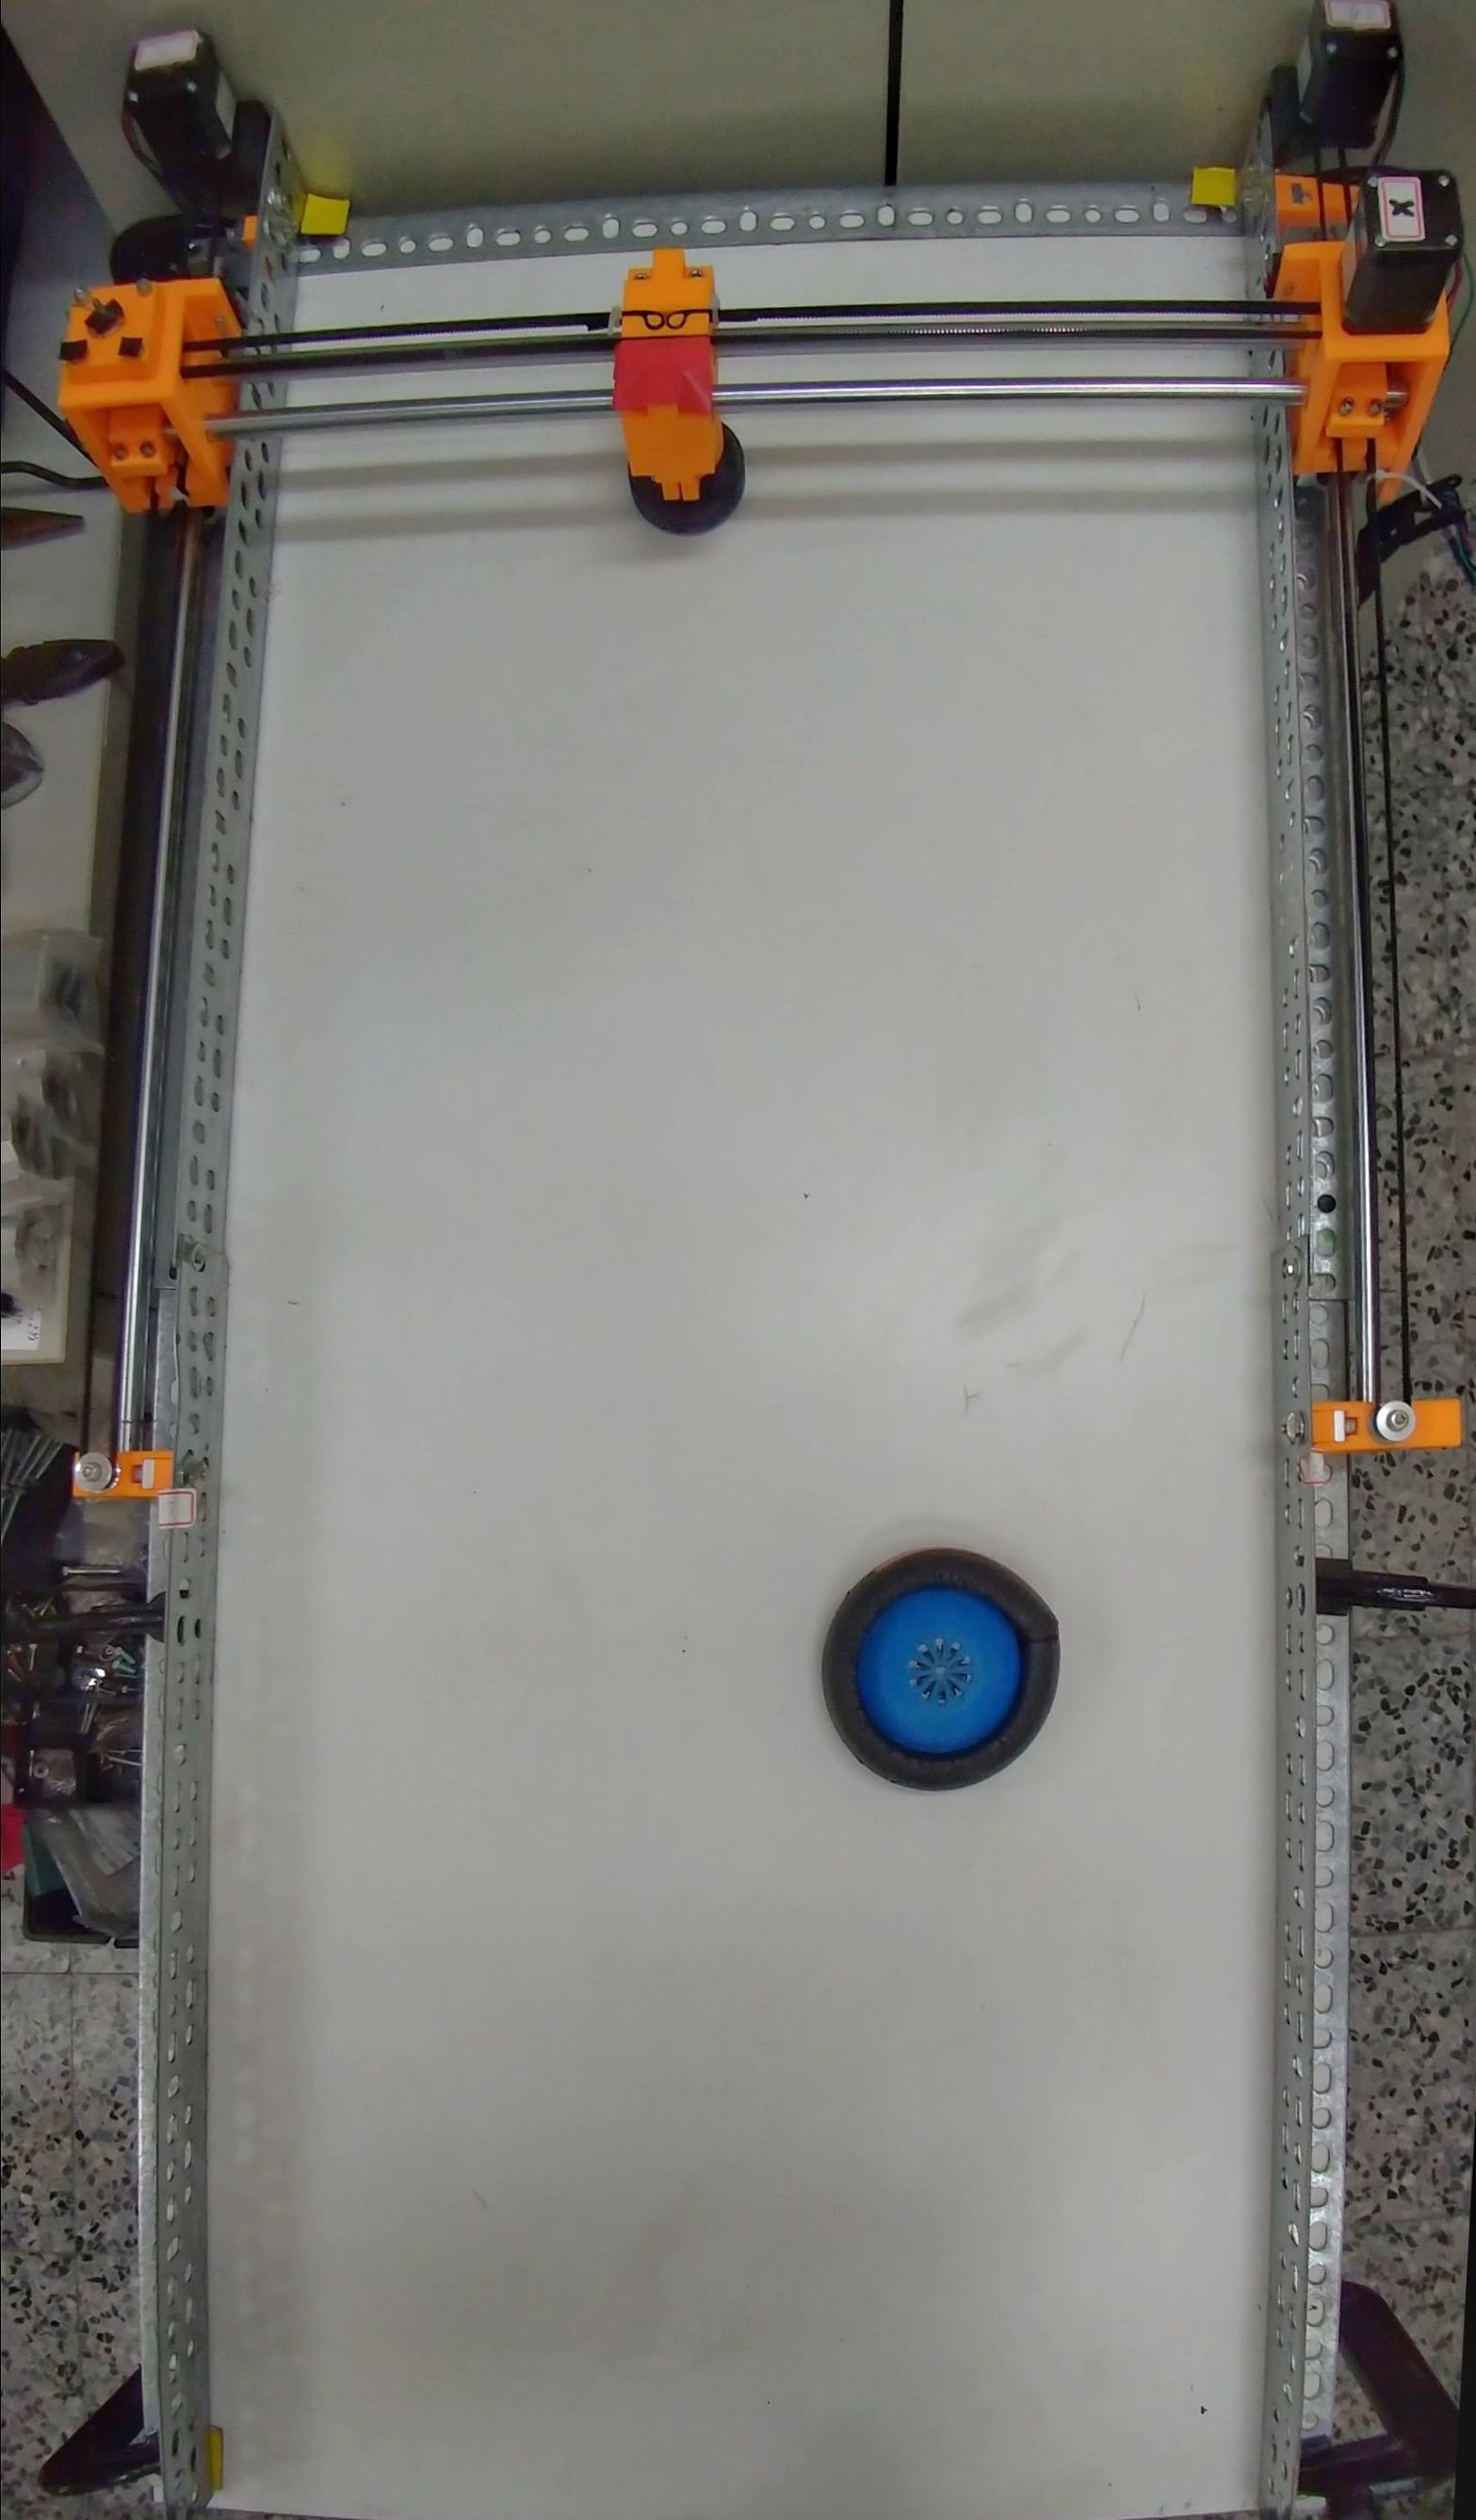
\includegraphics[width=4cm]{冰球機}
\caption{\Large 實體的冰球機}\label{fig.冰球機}
\end{minipage}
}
\subfigure{
\begin{minipage}[t]{0.3\linewidth}
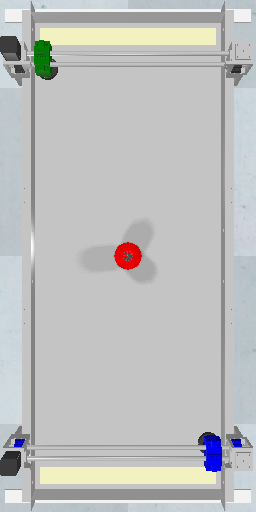
\includegraphics[width=4cm]{origin}
\caption{\Large 虛擬環境簡化後的冰球機}\label{fig.模擬冰球機}
\end{minipage}
}
\subfigure{
\begin{minipage}[t]{0.3\linewidth} 
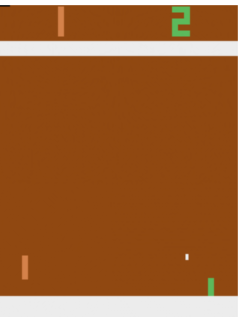
\includegraphics[width=4cm]{pong_gym}
\caption{\Large Gym的Pong game}\label{fig.pong_gym}
\end{minipage}
}
\end{center}
\end{figure}
\section{研究目的與方法}
 本研究分兩大部分,第一運用OpenAI Gym裡內建編譯的ATARI 2600遊戲Pong-v0,來作為訓練環境,加上強化學習的理論,測試不同演算法以訓練出最佳化的對打系統,第二換為CoppilaSim模擬環境並套用訓練程式,成為優化的對打機電系統。\\
 
 利用Gym的訓練環境來測試不同的算法所得到的訓練結果,比較不同算法、參數間的差異,並找出較適合Pong game的算法、參數,循序漸進提高環境的真實程度,來減少一開始就是以實體的方式測試所帶來硬體、程式、時間和金錢等成本。\\

 將Gym的訓練環境轉換到CoppilaSim模擬環境,利用貼近真實的模擬環境來修正在純程式的架構(Gym)與真實環境間的誤差,雖然CoppilaSim模擬環境與真實環境仍有些微的落差,兩者相比CoppilaSim的環境已非常貼近真實了,拉近了虛擬與現實間的距離,提高了實用性的價值。
\section{未來展望}
此專題希望能利用機械學習達到設計最佳化,並以其數據加入到對應虛擬環境進行演練,再以完整伺服器與網頁進行觀看、操控、更改環境參數,將以上綜合導入到實體機電系統上,實現機械學習在機電系統中的應用。且希望簡化設計過程加速整體設計流程,使其流程應用在各產業設計。
\section{規則說明}
 Pong game 的遊戲規則簡單,透過擊錘將球打入對方球門即得一分,只要其中一方得21分就結束該局。擊錘只能沿單方向來回移動來進行防守和進攻。\\
遊戲規則如下:
\begin{enumerate}
\item 球打入敵方即得一分。
\item 擊錘只單一方向移動。
\item 最快贏得21分者獲勝,並結束該局遊戲。
\end{enumerate}

\renewcommand{\baselinestretch}{0.5} %設定行距